\chapter{Conclusioni e possibili sviluppi}
\label{Conclusione}
%
I modelli sviluppati, nelle corrette condizioni di lavoro, soddisfano la necessità del calcolo in tempo reale imposto dalle condizioni di utilizzo. Il tempo di calcolo sull'\textit{hardware} del simulatore professionale si traduce in un ciclo di lavoro massimo del 4.3\% circa, garantendo quindi un ampio margine di sicurezza e dando la possibilità di aumentare la precisione del modello attraverso l'implementazione di modelli più complessi.

I modelli di contatto sviluppati garantiscono un tempo di esecuzione basso. In generale per qualità dell'\textit{output} generato e per tempo di compilazione il modello di contatto ponderato sull'area d'intersezione è da preferire. Esso infatti permette di rilevare ostacoli anche al di fuori dell'impronta di contatto garantendo quindi una descrizione qualitativamente maggiore del contatto tra lo pneumatico e la strada. Inoltre è opportuno settare lo \textit{switch} tra un modello di contatto e l'altro indicaticamente quanto i triangoli all'interno dell'ombra di contatto sono maggiori del prodotto tra il numero di dischi e il numero di punti di campionamento associati ad ogni disco. Considerando dunque le finalità principali e i test effettuati sul modello sviluppato, possiamo affermare la sua validità per i campi di utilizzo previsti.

Un punto critico sul quale è opportuno porre particolare attenzione è la rappresentazione del terreno. I \textit{file} \ac{RDF} hanno una struttura dati molto poco formale e solida. La mancanza di uno standard universalmente riconosciuto per questo formato rende impossibile implementare un \textit{parser} sufficientemente efficiente e la stabile per tutte le occasioni.

\begin{figure}
	\centering
	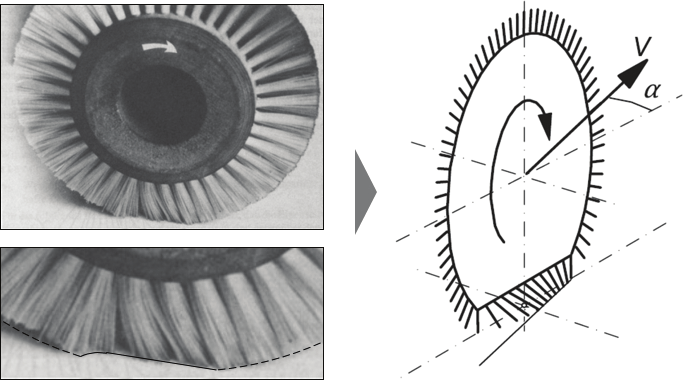
\includegraphics[width=0.7\linewidth]{Figures/brush_model}
	\caption{Schema strutturale del modello "a spazzola" (\textit{brush model}). }
	\label{brushmodel}
\end{figure}

Infine, bisogna certamente notare che la rappresentazione dello pneumatico è basato sul modello di Pacejka, ovvero un modello semi-empirico che non tiene conto dei fenomeni transitori. Sarà quindi una scelta obbligata passare ad una rappresentazione dello pneumatico mediante un modello fisico. Quest'ultimo, infatti, a seconda del grado di complessità, può tenere in considerazione alcuni dei fenomeni transitori che maggiormente influenzano la manovrabilità del veicolo. I modelli fisici sono quindi anche molto complessi. Lo pneumatico è modellato da divesi anelli circolari con punti di massa accoppiati anche in direzione laterale. Si tiene quindi conto del contatto in più punti e della distribuzione della pressione su tutta la larghezza della cintura. Importante sarà quindi valutare la possibilità di poter parallelizzare i processi di calcolo per diminuire i tempi di esecuzione.